\documentclass[11pt]{article}
\usepackage{amsmath,amsfonts}
\usepackage[numbers,sort&compress]{natbib}
\usepackage{times}
\usepackage[left=2.54cm,top=2.54cm,right=2.54cm,bottom=2.54cm,bindingoffset=0.0cm]{geometry}
\usepackage{setspace}
\usepackage{enumerate}
\usepackage{enumitem}
\usepackage{wrapfig}
\setcounter{secnumdepth}{0}
\usepackage{fullpage}
\usepackage{titlesec}
\titleformat{\section}{\large\bfseries}{\thesection}{1em}{}
\titleformat{\subsection}{\bfseries}{\thesubsection}{1em}{}
\usepackage{parskip} % skip paragraph indentations
\usepackage{lipsum}
\usepackage{hyperref}
\usepackage{graphicx}
\usepackage{amssymb}
\usepackage[x11names]{xcolor}
\usepackage{hyperref}
\usepackage{enumitem}
\usepackage{booktabs}
\usepackage{amsmath}
\usepackage{amssymb}
\usepackage{mathrsfs}
\usepackage{caption} \captionsetup[table]{singlelinecheck=false} %makes table captions left-justified
\usepackage{framed} % to add frames around comments
%\hypersetup{backref,colorlinks=false,
%    urlbordercolor=LightSkyBlue4,          % color of internal links
%    citebordercolor=SpringGreen4,        % color of links to bibliography
%    filebordercolor=magenta,      % color of file links
%    linkbordercolor=Red3, pdfborderstyle={/S/U/W 1.5}}
\newcommand{\Prob}[1]{\Pr{\left( #1 \right)}}
\newcommand{\q}[1]{``#1''} % easier way to get double quotes
\newcommand{\argmin}{\text{argmin}}
\usepackage{authblk} % for title page
\renewcommand\Affilfont{\fontsize{10}{10.8}\itshape}
\renewcommand\familydefault{\sfdefault} 
\usepackage{datetime2}
%\renewcommand{\dateseparator}{-}
\usepackage{atbegshi}% http://ctan.org/pkg/atbegshi -- removes blank page at start of doc
\AtBeginDocument{\AtBeginShipoutNext{\AtBeginShipoutDiscard}}
\setcounter{page}{0}

\lhead{Large groups and learning costs promote signal-based assessment} 


\begin{document}
\noindent
\title{Large groups and high learning costs promote the evolution of signal-based social assessment} 
\author{}
\date{} 
\maketitle

%New target journal: Proc B 
%instructions: http://rspb.royalsocietypublishing.org/author-information
% open access: https://royalsociety.org/journals/authors/open-access/

%%%%%%%%%%%%%%%%%%%%%%%%%%%%%%%%%%%%
\linenumbers

\section*{Lay summary}
%Animals that live in groups often need accurate information about their group mates, but there are several ways that this assessment can work. Some animals learn to recognize something about others, and sort individuals into categories or remember particular individuals, but others may learn general rules of thumb that apply to all individuals. We find that recognition learning is always more difficult than rule learning in large groups and when animals have poor memory. In these cases, it is better to learn about general rules of quality, rather than relying on learning about to recognize individuals.

% % TERMS:
% individual recognition vs signal-based assessment strategies
% categorical vs rule-based strategies for inferring quality from signal

% STYLE NOTES:
% - how to treat rule / rule of thumb?

%%%%%%%%%%%%%%%%%%%%%%%
\section*{Abstract}
%%%%%%%%%%%%%%%%%%%%%%%
%Animals in social groups benefit from having accurate information about their group mates. Different species have different methods for gathering this information: some animals recognize members of their groups as individuals, while others coarsely categorize conspecifics based on observable traits. In many animals, a property of interest, for example dominance or health, is correlated with an otherwise unimportant trait, which is then referred to as a badge of status. Much is known about the circumstances that promote the evolution of either individual recognition or a badge of status, but there are few studies that compare the effectiveness of the two systems of learning. In order to study how group size and cognitive abilities influence the effectiveness of both types of learning and to determine the circumstances under which one is preferable, we develop and analyze a simple model of an animal social group, in which animals learn by interacting with each other and by observing these interactions. Regardless of how the animals assess the quality of their group mates, we find that larger group sizes and longer memory windows make it easier to learn more accurately and more quickly. We also find that intermediate perceptive abilities maximize the effectiveness of learning about a badge of status and that observational learning is more beneficial for animals using individual recognition. Finally, we find that learning about a badge of status is less costly than individual recognition when animals live in large groups, have short memories, and have coarse perceptive abilities.



\textbf{Keywords:} badge, cognition, evolution, learning, recognition, signal, social groups

\newpage
%%%%%%%%%%%%%%%%%%%%%%%
\section*{Introduction} 
%%%%%%%%%%%%%%%%%%%%%%%
%% SOCIAL INFORMATION
Animals in social groups benefit from having accurate information about their group mates \citep{Seyfarth:2010bh}. For example, an animal can make a better decision about whom to fight if it knows something about the dominance ~\citep{Waal:1986ys,Cowlishaw:1990vn,Bergman:2003qf,Seyfarth:2005ve,Flack:2006uq,Hobson:2015uq} or resource holding potential~\citep{Rhijn:1980uq,Freeman:1985kl,Dick:1990cr,Lemel:1993ve,Part:1997ys} of the other members of its group. A female can  make a better decision about whom to mate with if she has some information about a male's likelihood of investing in parental care~\citep{Qvarnstrom:1997fk,McGlothlin:2007au,Olsen:2010uq} or his health~\citep{Folstad:1992kx,Loyau:2005nx}. In addition to affecting how animals make decisions about social interactions, the information that animals have about each other can affect the type of social structure that emerges in their group \citep{Dugatkin:2004hz,Hobson:2015uq,Brush:2018ss}. In order to understand the evolution of sociality, it is therefore important to understand the strategies animals use to make assessments of each other.  

%% SIGNAL-BASED ASSESSMENT
There are many examples of species in which one trait acts as a signal of another less visible trait. When the property of interest is an animal's resource holding potential, the signal is called a badge of status \citep{dawkins1978signals,Rohwer:1981vn,Rohwer:1982fk,Ripoll:2004vn,sheehan2016evotradeoff}. A classic example of this is provided by house sparrows (\emph{Passer domesticus}), in which the size of a male's bib is correlated with his dominance \citep{Veiga:1993fk,Veiga:1995ys}. Badges of status have also been demonstrated in several other species of birds (e.g., \citep{Remy:2010fk,Olsen:2010uq,Lemel:1993ve,Tibbetts:2009kx}), mammals (e.g., \citep{Gerald:2001zm}), reptiles (e.g., \citep{Fox:1990hd}), and insects (e.g., \citep{Tibbetts:2004kx}). Signals can also provide information about other properties. For example, some species of birds have signals that communicate their current health status \citep{Folstad:1992kx,Loyau:2005nx}. In humans, a smile may be a signal of a person's likelihood of cooperating \citep{Schug:2010be}. Once such a signal has evolved, animals can use the signals displayed by their peers to make estimates of the property of interest, be it resource holding potential, health, likelihood of cooperating, or anything else.

It is difficult to determine how animals actually use a signal to assess conspecifics. In order to prove that a trait is a quality signal, scientists usually identify a statistically significant linear relationship between the putative signal and a property of interest (e.g., \citep{Rohwer:1981vn,Rohwer:1982fk,Ripoll:2004vn,Tibbetts:2004kx}). Animals could use such a linear relationship as a rule dictating how to map a signal to a quality value. While it is often assumed that animals are born knowing this rule \citep{sheehan2016evotradeoff}, it is also plausible that they learn it over the course of interacting with conspecifics. Many cognitive processes in both humans and non-human animals are based on a categorical perception of the world \citep{Harnad:1990ux}. Both sound (e.g., \citep{Wyttenbach:1996wj,Nelson:1989rt}; reviewed in \citep{Bornstein:1987ec,Ehret:1987jh}) and color (e.g., \citep{Lim:2016ye}; reviewed in \citep{Bornstein:1987ec}) have been demonstrated to be perceived categorically by different types of animals. Categorization provides an alternative way for animals to make inferences about the quality of their peers based on the signals they display. For example, a zebra finch might categorize conspecifics by whether their bills are more red or orange and subsequently learn that birds with red bills have high resource holding potential and birds with orange bills have low resource holding potential TKTK.   
 
%% INDIVIDUAL RECOGNITION
In contrast to using signals to assess one's peers, an animal can simply recognize and learn about each other animal individually \citep{sheehan2016evotradeoff}. Individual recognition has been demonstrated in many species and can be based on visual, olfactory, or auditory traits (reviewed in \citep{Tibbetts2007IndividualDifferent}). An animal with imperfect cognitive abilities may confuse similar conspecifics. As an animal's ability to discriminate becomes worse, it will confuse more and more animals and may resort to learning about them categorically. Individual recognition can therefore be thought of as extremely fine categorical recognition \citep{Barnard:1979fk}. Such a spectrum from coarse-grained to fine-grained perceptive abilities can be seen in some real world examples. Within paper wasps, some species distinguish between other wasps based on the number of black patches on their face, a relatively coarse trait \citep{Tibbetts:2004kx}, whereas in other species, wasps can recognize specific individuals based on their unique facial patterns \citep{Tibbetts:2002ys}. 

%% BIG UNKNOWN QUESTION
Regardless of how the assessment is being made, there are two things that have to be present in order to have a functional system of social assessment: (1) a trait that is used as either a quality signal or an identity signal and (2) an assessment strategy that is either signal-based or recognition-based.  On the signal side, much work has been done to understand when quality signals or badges of status should be expected to evolve (e.g., \citep{Whitfield:1987tg,Rohwer:1975fk,Rohwer:1982fk,Dawkins:1991ly,Johnstone:1995vn,Lachmann:1998fk,Tibbetts:2009kx}). For example, in birds, badges of status seem to evolve in species that live in large and fluid groups in the non-breeding season \citep{Tibbetts:2009kx}. There are also many studies that have identified the circumstances that facilitate the evolution of identity signals \citep{Rohwer:1975fk,Whitfield:1987tg,Sheehan:2009we,Pollard:2011te,Sheehan:2014fk}. In particular, identity signals are more likely to evolve in species that have complex social structures or highly territorial behavior \citep{Tibbetts2007IndividualDifferent}. On the assessment side, we do know some factors that should facilitate the evolution of individual recognition. For example, there needs to be sufficient variability in the trait that will be used as an identity signal \citep{Sheehan:2014fk}. Individual recognition is also more likely to evolve in species where animals can avoid costly fights by recognizing which conspecifics to avoid \citep{DEttorre:2005nu}.  \citet{sheehan2016evotradeoff} pursued a thought experiment in which they compared the errors and learning time associated with quality signaling and individual recognition and made predictions about when one or the other would be preferable. They predicted that signal-based assessment strategies will not be affected by the number of interactions a pair of animals engages in or the size of the social group, whereas individual recognition should improve over time and become more difficult in larger groups \citep{sheehan2016evotradeoff}. They also predicted that individual recognition should be preferable in small groups when animals have many opportunities to learn about each other \citep{sheehan2016evotradeoff}. Quantitative support of these qualitative predictions was left for future work. Despite the fact that \citet{sheehan2016evotradeoff} identified this as an important problem, there are few modeling studies that compare the efficacy of signal-based assessment to that of individual recognition. 

%%MEMORY
Whether a signal-based or recognition-based assessment strategy is preferable will depend on several factors. As we described above, individual recognition can only work if the animals have sufficiently fine perceptive abilities. There are other cognitive constraints that are important for understanding which type of assessment method is best. An animal's memory can limit its ability to remember its assessments of its peers. 
If animals use a linear rule to make assessments about their peers, there are essentially two parameters to remember: the slope and intercept of the line. Similarly, if animals categorize their peers, they only have to remember as many pieces of information as there are categories. However, if animals use individual recognition, they must remember the quality of each of their peers, which can become prohibitively difficult in large groups  \citep{Rohwer:1982fk,Solberg:1997uq}. It can become even more problematic if animals have to remember the relationships between pairs of other animals ~\citep{Seyfarth2015SocialCognition}. Even humans are thought to be limited in terms of the number of people we can recognize. Previous work has hypothesized that humans can only remember the faces of about 150 people \citep{Dunbar:1993zr,Hill:2003ly}, which may have limited group size over the course of human evolution~\citep{Dunbar:1992ys,Dunbar:1993zr}. 

%%UTILITY OF ASSESSMENT
The final factor in understanding when which type of assessment will evolve is being able to quantify the costs and benefits of using either strategy. Animals assess each other and use information about their group mates to decide how to interact with them in the future. Therefore, if animals learn about each other inaccurately, they will make inappropriate decisions and incur costs. On the other hand, individuals are constrained in the total amount of effort and time that they can devote to assessing each other \citep{MacIver:2010ve}. Additionally, if interactions are aggressive, engaging in more interactions than necessary can lead to injury. The overall cost of using a particular assessment strategy will be a combination of the costs of the errors made and the time it took to make the assessment. There is an inherent tradeoff between accuracy and speed because waiting longer and gathering more information improves the accuracy of an animal's assessment.  This tradeoff will vary from species to species and will affect which assessment strategy is preferable.  

Our goal in this paper is to understand when different types of assessment strategies will evolve by comparing the costs of signal-based assessment strategies and individual recognition.  In order to do so, we developed an agent-based model of an animal social group in which animals assess each other's quality through dyadic interactions and incur costs based on these assessments. We first analyze how group size, cognitive abilities, and the cost of the time spent assessing influence each assessment strategies. We then identify the cognitive traits that optimize an animal's ability to assess its peers via categorical and individual recognition. Finally, we identify the circumstances under which each strategy is preferable. In general our results conform to the predictions of \citet{sheehan2016evotradeoff}, although we extend their thought experiment by analyzing both innate \emph{and} learned signal-based assessment strategies and considering a categorical assessment strategy that grades into individual recognition. 
 

%%%%%%%%%%%%%%%%%%%%%%%
\section*{Model } 
%%%%%%%%%%%%%%%%%%%%%%%

%\subsection{Interactions and quality assessment}
We consider with a group of animals containing $N$ individuals (see Table~\ref{tab:vars} for parameter descriptions). We assign each animal a quality value, $q_i$, and a signal, $s_i$. Quality can be thought of, for example, as fighting ability, resource holding potential, body size, body condition, or any other property about which it would be beneficial to have accurate information and which it may be difficult to estimate without interacting with an animal. While the types of traits that can be used either as quality signals or for individual recognition are likely different \citep{Dale:2001dv}, we assume that the animals vary in a single visible trait, which can be used either as a quality signal or for individual recognition and which can be measured without having to interact with an animal.  

Specifically, we draw quality values $\{q_1,\dots,q_N\}$ from a normal distribution with mean $0$ and standard deviation $\sigma_\text{q}$. We then generate $N$ signal values $\{s_i\}$ such that 
%$\min_i{s_i}\approx -1$, $\max_i{s_i}\approx 1$, and 
$\max_i\{s_i\}-\min_i\{s_i\}=2$ and the sample correlation between $\{q_i\}$ and $\{s_i\}$ is precisely $\rho$. 
The higher $\rho$ is, the more informative the signal is about the underlying quality of the animals. The animals then use these signals to assess the quality of their group mates.

We consider two main ways in which animals assess each other: (1) a linear rule that maps signal to quality, which can be either innate or learned, and (2) categorization, which becomes into individual recognition when the animals can perceive small enough differences to be able to distinguish all of their peers. Under each system, the animals interact and assess each other for $T$ timesteps. At each point in time, two animals, $i$ and $j$, are chosen randomly to interact. Through this interaction, each receive noisy information about the other's quality: $i$ perceives $j$'s quality to be $\hat{q}_j=q_j+\xi$, where $\xi$ is drawn from a normal distribution with mean $0$ and standard deviation $\sigma_\xi$.  Additionally, every animal makes an assessment of every other at each point in time. We will write $a_{ij}(t)$ for the assessment that animal $i$ has of animal $j$ at timestep $t$. We now describe each assessment strategy system in detail.

%XXX MOVE TO DISCUSSION
Observational learning is known to be important in many systems (e.g., \citep{Freeman:1985kl,Holekamp:1991nx,Schaik:2011oq,Hobson:2015uq,Seyfarth2015SocialCognition}). However, we are interested in the inherent costs and benefits of the different assessment strategies and do not consider observational learning here. 


\subsection*{Linear rule}
We first describe animals that use a linear rule to infer quality from signal. In this case, each animal's assessment is given by
\begin{equation*}
a_{ij}(t)=m_i(t)s_j+b_i(t),
\end{equation*}
where $m_i(t)$ and $b_i(t)$ are the slope and intercept that $i$ believes describe the linear relationship between signal and quality at timestep $t$. When the rule is innate, these parameters do not change over time and they are the same for all animals in the group. An innate rule has presumably evolved over time to describe the average relationship between signal and quality. To model this, we generate $10,000$ groups with quality and signal values as described above. In each group, we find the slope $m$ and intercept $b$ of the best-fitting line through the points given by $\{s_i\}$ on the x-axis and $\{q_i\}$ on the y-axis. We then take the average of these over all $10,000$ groups and assume that all individuals in the group use $m_i(t)=\bar{m}$ and $b_i(t)=\bar{b}$ for all $i$ and all $t$. Thus, there is no learning and animals can use this rule immediately. 

%\subsection*{Learned rule}
We also allow animals to learn a rule to assess each other's quality. In this case, all members of the group are initially naive and have no estimate of the slope and intercept of the signal-quality relationship. The animals have a ``memory window" $w$ such that each animal remembers any interactions that have occurred within the last $w$ timesteps. From each of these recent interactions, an animal $i$ stores the signal of its opponent, $s_j$, as well as noisy information about its quality, $\hat{q}_j$.  Then $m_i(t)$ and $b_i(t)$ are the slope and intercept from the best-fitting line through the points given by the observed $\{s_j\}$ on the x-axis and the observed $\{\hat{q}_j\}$ on the y-axis.   

\subsection*{Categorization}
We next describe animals that perceive their conspecifics' signals categorically. In this case, the way animals categorize their peers depends on the magnitude of the differences in signals they can perceive. Specifically, an animal can only distinguish between two other animals $j$ and $k$ if $|s_j-s_k|>\delta$, that is, if their signals are sufficiently different. If the animals have fine perceptive abilities, the parameter $\delta$ will be small, and if the animals have coarse perceptive abilities, the parameter $\delta$ will be large. For example, if $\delta$ is be large, an animal can only discriminate among animals with small, medium, and large signals, and the best it can do is to learn about the quality of all animals in each of these three categories. On the other hand, if $\delta=0$, an animal can discriminate among every individual in its group and is capable of individual recognition. We will refer to the strategy of using categorization with $\delta=0$ as individual recognition below.

Before any interactions take place, each animal in the group divides its peers into categories. It does so by picking another animal, $j$, at random. All animals whose signals are within $\delta/2$ of $s_j$ are put in the same category. Then the focal animal picks an uncategorized animal at random, $k$, forming a second category of all uncategorized animals whose signals are within $\delta/2$ of $s_k$. The process continues until every animal in the group has been assigned a category. The parameter $\delta$ can therefore be thought of as ``category width."  Different animals will categorize the group differently and may perceive different numbers of categories. Figure \ref{cats_ex} shows one example of this process for various values of $\delta$. Since we analyzed the effects of several parameters, we chose a representative set of values rather than exploring every possible value of each parameter. In particular, we allow $\delta$ to take on the values $0$, $0.25$, $0.5$, $0.75$, and $1$.

%\subsection*{Updating assessments}
As with the learned rule above, at first, the group consists entirely of naive animals: at $t=0$, no animal has an opinion of any other. Again, each animal has a memory window $w$ such that it remembers categories it has encountered in the last $w$ timesteps and forgets its opinion of categories it has not interacted with so recently. Each animal then updates its assessment of the other to be the weighted average of its old estimate and the new information it has received. Specifically, if $i$ already has an assessment of $j$'s category, its new assessment of the category
\begin{equation*}
a_{ij}(t+1)=(1-r)a_{ij}(t)+r\hat{q}_j,
\end{equation*}
where $r$ is the ``updating rate" describing how much each animal changes its assessment based on the interaction. As with $\delta$, we choose a representative set of values of $r$ to explore, specifically, $0.05$, $0.1$, $0.25$, and $0.5$. Animal $i$ simultaneously updates its opinions of all the other animals in the same category as $j$.
If $i$ has not previously interacted with animals in $j$'s category or if $i$ has forgotten about the category, its new estimate of the category is
\begin{equation*}
a_{ij}(t+1)=r\hat{q}_j.
\end{equation*}
%In words, an animal's baseline opinion of a stranger is $0$, the average quality value of any group. 

When $\delta=0$, there are as many ``categories" as there are animals and the animals can be said to be using individual recognition. As category width increases, the average number of categories animals recognize decreases (Figure \ref{num_cat}). According to \citet{sheehan2016evotradeoff}, what distinguishes an assessment strategy that relies on quality signals from individual recognition is that, with a quality signal, an animal can know something about a conspecific based solely on the signal it displays without having had to interact with it. In our model, this is true for animals using categorization with category width $\delta>0$, as well as for animals using either an innate or learned rule (Figure \ref{schematic}). In other words, both the categorization and rule strategies we analyze can be considered signal-based assessment strategies that differ in whether they are innate or learned and in how animals infer quality from signal. 
 
\subsection{Assessment errors }
For each assessment system and each combination of parameters, we simulate $25$ groups undergoing the processes just described.  To quantify how well the animals assess each other, we measure how accurately and how quickly they assess each other's quality. The error of animal $i$'s assessment of animal $j$ at time $t$ is $e_{ij}(t)=|a_{ij}(t)-q_j|$. For a given combination of parameters, we take the average error that any animal makes in its assessments of the rest of its group over all groups, 
\begin{equation*}
\epsilon(t) = \frac{\sum_{\text{groups}}\sum_i\sum_{j\in \mathscr{O}_i(t)}e_{ij}(t)}{25N|\mathscr{O}_i(t)|},
\end{equation*}
where $\mathscr{O}_i(t)$ is the set of animals about whom $i$ has an opinion at time $t$.

In Figure \ref{learning_curves} we show representative examples of how the average error of animals using each assessment system changes over time.  For animals using either a learned rule or categorization, as the animals learn about each other, $\epsilon(t)$ decreases until it reaches an asymptote (Figure \ref{learning_curves}). At first, animals are more or less guessing about the quality of their peers, which results in a high average error. When learning is difficult, for example because the animals' memory is poor or there are many animals to learn about, the average error barely decreases from its initially high level (Figure \ref{learning_curves}). When learning is easier, for example because the animals can remember more interactions, because there are fewer animals to learn about, or because the signal becomes more informative, average error decreases over time and can even approach $0$ (Figure \ref{learning_curves}).  

\subsection{Assessment costs }
We are interested in identifying which assessment strategy is least costly, as this is the strategy we might expect to evolve. To do so, we must measure the cost associated with each assessment strategy. Animals incur costs when they have inaccurate estimates of their peers' quality and by continuing to spend time learning about each other when they could be engaging in other activities. We thus quantify the cost of learning at time $t$ as 
\begin{equation*}
C(t) = 2c\epsilon(t) +(1-c)\frac{t}{T}.
\end{equation*}  
The parameter $c$ ranges from $0$ to $1$ and quantifies the tradeoff between accuracy and speed: when $c$ is close to $1$, errors are more costly and when $c$ is close to $0$, the time spent learning is more costly. The factors of $2$ and $1/T$ ensure that the two costs are on the same scale, namely between $0$ and $1$. 
The cost function initially decreases, reaches a minimum, and either stays constant at that value or starts to increase (Figure XX). 

As we will show, increasing an animal's memory always improves how accurately it can learn. However, it may be costly to invest in improved memory. Rather than using an arbitrary cost function to describe these costs and finding the optimal memory window, we treat memory window as a variable that affects how well the animals can learn and what learning strategies they should use. 
%As we show later, it is sometimes beneficial for an animal to group its peers into categories based on the signals they display. Similarly, different updating rates are beneficial in different circumstances.

\subsection{Optimization }
There are strategies animals can use to minimize their costs within a particular assessment strategy. In order to study the evolution of the assessment strategies more broadly, we first study the evolution of each assessment strategy individually. While group size $N$ and signal-quality correlation $\rho$ may evolve over time, we assume that they are fixed on the timescales we consider. Similarly, memory $w$ may evolve over time, but we consider it as a fixed parameter in order to analyze the effects of memory on the evolution of assessment strategies. 

One strategy that animals \emph{can} vary is how many interactions they engage in before they stop learning. The animals should stop interacting for the sake of learning when the cost function $C(t)$ first reaches its minimum value (Figure XX). We refer to the number of interactions at which this occurs as the stopping time $\tau$. In other words, $C(\tau)$ is the minimum cost that can be incurred for a given set of parameters. When $c$ is close to $1$, the animals will keep learning to improve their accuracy and $\tau$ will be high, whereas when $c$ is close to $0$, taking time to learn is costly and $\tau$ will be low. For animals using an innate rule, $\tau$ is always equal to $1$ because they do not engage in learning and cannot improve their assessments by engaging in more interactions. 
% QUESTION: above, should the "c" be upper or lowercase here? "which is the number of interactions it takes before $C$ first reaches its minimum value" (was upper, but I think it should be lower??) 
% ANSWER: in that case it should be C, the cost function itself
% Memory is also costly 

Animals using categorization may also be able to evolve or optimize the values of $\delta$ an $r$ to minimize their costs. We first fix the group size $N$, signal-quality correlation $\rho$, memory window $w$, and cost of errors $c$. Then, for every combination of $\delta$ and $r$ we find the stopping time $\tau$ and therefore the minimum possible cost $C(\tau)$. Finally, we find the combination of $\delta$ and $r$ that minimizes $C(\tau)$. These are the parameters we would expect to evolve in a population using categorization as its assessment strategy. 

To compare all assessment strategies, for a given group size $N$ signal-quality correlation $\rho$, memory window $w$, and cost of errors $c$, we compare the cost of learning for animals using an innate rule ($C(1)$, which does not depend on $w$), for animals using a learned rule ($C(\tau)$), and for animals using categorization ($C(\tau)$ with optimized $\delta$ and $r$). We would expect that the assessment system with the lowest cost would invade a population using either of the other two systems.

%There are six important parameters in our model: group size $N$, the correlation between signal and quality $\rho$, memory window $w$, category width $\delta$, updating rate $r$, and stopping time $\tau$.  

The entire model was written in R and all model code will be released on publication on Github.

%%%%%%%%%%%%%%%%%%%%
\section*{Results}
%%%%%%%%%%%%%%%%%%%%
\subsection*{The effects of group size and cognitive abilities on learning}
We first analyze how average error $\epsilon(\tau)$ and stopping time $\tau$ depend on group size $N$, signal-quality correlation $\rho$, memory window $w$, category width $\delta$, updating rate $r$.

For animals using the innate rule, there is no learning involved, so memory, category width, and updating rate are irrelevant. In this case, the error with which animals can assess their group mates is essentially constant as a function of group size and is lower when the signal-quality correlation is higher (Figure \ref{parameters}A). As explained above, for animals using the innate rule, stopping time $\tau$ is always equal to $1$.

In contrast to the innate rule, animals using a learned rule or recognition (i.e. categorization with $\delta=0$) must spend time learning about their peers. For animals using these assessment strategies, the average of the animals' assessments increases as group size increases (Figure \ref{parameters}A). 
%This can also be seen by comparing the panels in Figure \ref{learning_curves}). 
They also tend to take more time to learn as group size increases (Figure \ref{parameters}E), although stopping time ($\tau$) does decrease as a function of group size when learning is so difficult that it is not worth spending time on (Figure~\ref{parameters}E, red solid line). Assessment errors decrease (Figure \ref{parameters}B) and stopping time increases (Figure~\ref{parameters}F) as memory window ($w$) increases, although these effect is stronger for animals using recognition than for those using a learned rule (compare the solid and dashed lines in Figure \ref{parameters}B and F).  Animals using a learned rule or recognition with a category width greater than $0$ (i.e., not individual recognition) make smaller errors when the the signal and quality are more strongly correlated (compare the solid and dashed curves in Figure \ref{parameters}A-D). In summary, the effects of group size ($N$), memory window ($w$), and signal-quality correlation ($\rho$) on learning speed and learning accuracy and are intuitive and confirm that our model is a reasonable description of some of the basic properties of a real social system. 
 
For animals using categorization, when memory is poor, increasing the updating rate $r$ decreases error (the red curve in Figure \ref{parameters}C). This is because a higher updating rate helps animals form a somewhat accurate assessment of a peer before they forget past interactions. However, when animals have short memories, increasing the updating rate \emph{increases} errors (Figure XX), showing that individuals benefit from avoiding updating their assessment based on noisy information and benefit from incorporating new information slowly. Increasing the updating rate tends to decrease stopping time (Figure \ref{parameters}G): an animal will reach asymptotic assessments of its peers more quickly if it incorporates new information more readily. The interaction between memory window and updating rate on error and stopping time is shown in Figure \ref{interactions}.
 
For animals using categorization, when the signal is almost perfectly correlated with quality ($\rho$=0.99) and animals have short memories, an intermediate category width minimizes error (the blue curve in Figure~\ref{parameters}D). In other words, within the categorization strategy, it is using categories that contain more than one animal is sometimes more accurate than using individual recognition. This pattern can be explained as follows. Regardless of the signal-quality correlation, as category width increases, the number of animals in a given category also increases (Figure \ref{num_cat}). The first consequence of this is that an animal trying to learn about a given category will encounter it more often, and be less likely to forget its opinion of it before its memory window lapses. This tends to decrease the error with which animals can learn about their peers. The second consequence is that each time an animal encounters a category it extrapolates the information it gathers to more animals. This ``confusion" tends to increase learning error. When the badge is poorly correlated with quality, this increase in error due to increased confusion is much greater than the decrease in error due to a lower chance of forgetting. Therefore, as category width increases error increases as well. However, when the badge is highly correlated with quality, the increase in error due to increased confusion is much less pronounced because animals with similar badges do actually have similar quality values. Therefore, as category width increases, at first error decreases, because of the reduced probability of forgetting, while later error increases, because of increased confusion. When the animals have a long memory window, increasing category width always increases overall error because there is no chance of forgetting what has been learned (Figure~\ref{interactions}). 

\subsection*{Optimal learning strategies for animals using categorization}
We next analyze the optimal learning strategies, i.e. stopping time $\tau$, updating rate $r$, and category width $\delta$, for animals using categorization. As the cost of errors ($c$) increases, the optimal stopping time increases: animals should spend longer learning in order to acquire more information (Figure \ref{optimization}A-C, see also Figure \ref{time}). This is also true for animals using a learned rule (Figure XX). As the cost of errors increases, the optimal updating rate decreases: again, animals should spend longer learning and incorporate noisy information less readily (Figure \ref{optimization}D-F, see also Figure \ref{l}). In large groups or when memory window is short, animals should always use the highest updating rate (Figure \ref{optimization}D-F, see also Figure \ref{l}). 

Animals should use a category width greater than $0$ when errors are not very costly, when memory window is short, or when group size is large (Figure \ref{optimization}G-I). Under these circumstances, rather than focusing on the individual identity of their peers, the animals should categorize the rest of their group based on the signals they display and assess all of the animals in each category simultaneously. This is only true when the signal-quality correlation is quite high (e.g., $\rho=0.99$) (Figure \ref{delta}). Animals should instead using a category width equal to $0$, i.e. individual recognition, when errors are very costly, when memory window is long, and when group size is small (Figure \ref{optimization}G-I) and whenever the signal-quality correlation is not very high (Figure \ref{delta}). 

When animals use these optimal strategies---stopping time, updating rate, and category width---the error with which animals assess their peers is smallest when group size is small, when the cost of errors is high, and when memory window is high (Figure \ref{optimization}J-L). Figure \ref{optimization} shows optimal stopping time, updating rate, and category width when the signal-quality correlation is quite high ($\rho=0.99$). Results for lower values of $\rho$ are shown in Figures \ref{time}-\ref{error}.

\subsection*{Optimal assessment strategy}
Having found the optimal parameters for animals using categorization, we finally compare the overall costs of using each assessment strategy. Remember that the overall cost of using a strategy is a weighted average of the error with which animals can assess their peers and the number of interactions it takes to reach an accurate assessment. First, we compare the two learned strategies: categorization with optimized parameters and a learned rule with optimized stopping time. For those parameters where using category width greater than $0$ is optimal, categorization is never better than the learned rule (Figure \ref{comparison}). There are parameters, however, where using individual recognition is optimal and where recognition is less costly than the learned rule. Specifically, recognition is less costly than the learned rule when the signal-quality correlation is not very high, when the group size is small, and when animals have a long memory (Figure \ref{comparison}). Recognition is also favored when errors are very costly (Figure \ref{comparison}). 

When we compare all three assessment strategies, we find a similar pattern: recognition is the best of all three strategies in small groups, when animals have long memories, and when errors are costly (Figure \ref{best}). In other words, for animals that live in small groups, that have long memories, or that need to make accurate assessments of their peeers, it is preferable to invest in individual recognition than in a signal-based assessment strategy. Of the parameters where a rule is preferable, a innate rule is preferable to a learned rule only when group size is large ($N=100$) and the memory window is very short ($w\leq500$) (Figure \ref{optimization}). There are large regions of parameter space where all three assessment strategies perform almost equally (the purple regions in Figure \ref{optimization}).
%This agrees with predictions made by Sheehan et al. Whether learning about categories or a rule is easier is left for future research.

%%%%%%%%%%%%%%%%%
\section*{Discussion}
%%%%%%%%%%%%%%%%%
%to put somewhere: 
We find that the how strongly the signal is correlated with the property of interest determines whether a learned or innate rule is better. Whether animals use a learned or innate strategy for inferring quality from signal can in turn affect the evolution of the signal itself \citep{Kamo:2002vi}. A complete understanding of the evolution of social assessment will require considering the full feedback loop, that is including both the effect of the signal on the evolution of the assessment strategy and the effect of the assessment strategy on the evolution of the signal.


% Study question, restated/reframed
Having an accurate assessment of the quality of one's conspecifics is important in many contexts, but the conditions under which different assessment strategies may be favored is not well understood. Here, we modeled quality assessment in social groups, with animals using either a signal, which allows them to infer the quality of an unknown animal, or individual recognition, which allows them to learn about each particular individual. We considered three signal-based assessment strategies: an innate linear rule mapping signal to quality, a learned rule, and categorization of signals. Our goal was to better understand the costs and benefits of each system and the conditions under which each system might be favored. 

\subsection*{The effect of group size and cognition on learning} 

Smaller groups and longer memory duration make it easier to learn in each system, which is consistent with general intuition. While decreasing group size led to lower error and faster learning in both systems, the effect of group size on error and learning time is much greater in the individual recognition system than the categorical badge system. We also find that agents using the badge system learn more quickly and accurately when there is a strong correlation between the signal and quality. While the correlation values we use are a bit higher than those estimated in species for which this data has been collected (e.g., paper wasps \citep{Tibbetts:2004kx}, house sparrows \citep{Veiga:1993fk}, swamp sparrows \citep{Olsen:2010uq}, see Table \ref{corr_examples} for details), our model shows that even with a moderate correlation the badge system is an effective way to learn about one's group mates. These finding agree with the predictions of \citet{sheehan2016evotradeoff}, although they focused on animals that already have an innate knowledge of what a badge means, rather than ones that were required to learn about its meaning over time.


We also find that animals using the badge system minimize both the error with which they learn and their learning time by having a moderate ability to discriminate between different badges (i.e., by using an intermediate category width), as long as the badge is highly correlated with the underlying quality. This is somewhat counterintuitive as one might expect that it would always be advantageous to improve one's cognitive abilities. Our finding is related to the bias-variance tradeoff in statistics and machine learning: as a statistical model becomes more complex, it is more likely that its predictions will be accurate, but its predictions become more contingent on the training set and are therefore more variable \citep{Domingos:2000cr,Briscoe:2011nx}. Similarly, as animals increase the number of categories into which they place their peers, it becomes easier for them to learn accurately about each of those categories, but they forget their assessments more often and therefore have more variable assessments over time. %LIZ: I have "oooooo, nice" in my notes for this paragraph!!!

In our model, we assume that there is a continuously distributed signal that is lumped into categories based on the perceptive abilities of the receivers of the signal. Instead of a continuously distributed signal, there are systems in which subsets animals with similar quality values exhibit the same signal, so only a discrete set of signals is available to the receivers \citep{Johnstone:1994uq}. Theoretical models show that using a discrete set of signals, rather than a continuous distribution, can stabilize a signaling system. In some models, when receivers of the signal are error prone, equilibrium signaling strategies only includes a finite number of signals \citep{Grafen:1993kx,Johnstone:1994uq}. In a model that allows for multiple qualities to be communicated via multiple signals, it is also the case that animals with different quality values could display the same signals \citep{Johnstone:1995vn}. In another model, allowing for such ``pooled" signals increases the likelihood of finding a signaling equilibrium \citep{Lachmann:1998fk}. We find that perceiving a discrete set of categories can make it easier for a receiver to learn about the signals, which is further evidence that discrete signals are likely to be advantageous in many natural systems.


One explanation for why animals have imperfect cognition is that there are costs involved in improving their cognition \citep{Dunbar:1992ys,Laughlin:1998ly,Laughlin:2001qf,Gavrilets:2006fk,MacIver:2010ve}. However, our results suggest that imperfect cognition itself may be adaptive. This may explain empirical examples of imperfect cognition (e.g., \citep{Kikuchi:2010ys}).
Other studies have also found that the most advanced cognitive strategies are not always optimal \citep{Stephens:1991fk,Kerr:2003vn,Dunlap:2009vn}. Our work therefore contributes to our growing understanding of the circumstances that do not lead to the evolution of sophisticated cognition.

When we allow the animals in our model to learn by observing interactions between other pairs of animals, only animals using individual recognition benefit from being able to learn more quickly and accurately. While previous work has shown the benefits of observational learning \citep{Freeman:1985kl,Holekamp:1991nx,Schaik:2011oq}, our study shows that the benefits depend on how learning occurs in the first place. Our finding is somewhat surprising because one might expect that making more observations helps animals using the badge system to make up for the deficit inherent in their categorical method of learning. Several species are capable of both observational learning and individual recognition (e.g., chimpanzees \citep{Parr:2000hc,Hopper:2008bh}, dolphins \citep{Sayigh:1999bs,Krutzen:2005ij}). One explanation of these shared traits is that only species with advanced social cognition would be capable of both individual recognition and observational learning require. However, our results suggest another explanation: it is precisely in those species that use individual recognition that observational learning is most advantageous.

\subsection*{The overall costs of learning} %LIZ comment: tried to clarify this a bit more -- I was actually forgetting how the costs mapped to cognition (!!) so I added a little reminder here
In our model, we defined the total cost of learning as a combination of five sources of cost (error, time, frequency of observations, memory window, and category width). Of these, animals can invest in increasing their cognitive abilities in two ways: by increasing their perceptive abilities so they can better discriminate among signal categories (decreased category width) or by increasing their memory capabilities (increased memory window). Depending on how quickly the inherent costs of these cognitive traits increase in our model, the total cost of learning is minimized by either not investing at all in additional cognition, or by investing in moderate cognition (e.g., either with an intermediate memory window or an intermediate category width). We find no cases where the benefits of using the most advanced cognitive ability available, either a very long memory window (perfect memory) or category width equal to $0$ (perfect signal discrimination), outweighed the cost of using such a trait. This finding reinforces previous studies that showed how difficult it is for advanced cognition to evolve \citep{Kerr:2003vn}.


\subsection*{The evolution of assessment systems} %temp heading

We find that learning about a badge of status is less costly than using individual recognition when the animals live in large groups, have short memories, and coarse perceptive abilities. In our model, the badge of status is preferable in any group with more than $50$ members (except when the animals have infinite memory, in which case the threshold becomes $70$ instead). This finding agrees with previous studies that found that individual recognition is most useful in small groups \citep{Veiga:1993fk}. In particular, Dunbar has argued that early human societies were limited by the number of other people a person can effectively learn about \citep{Dunbar:1993zr,Hill:2003ly}. While our threshold group size is not identical to his threshold of a group size of 150, they are of the same order of magnitude. Our finding also agrees with previous studies of badges of quality, which have found that badges are more likely to evolve in large groups with fluid social systems \citep{Rohwer:1975fk,Tibbetts:2009kx}. By explicitly comparing the two systems, we have generated a prediction about the types of groups and species in which we expect one or the other system to evolve. Testing this prediction is left for future work. 

 
\subsection*{Future work and conclusion}
 
By studying a simple model of sociality, we were able to identify the conditions under which two assessment systems are most effective and determine the conditions under which one or the other system should evolve. There are further steps towards improving the realism of the model that will also improve our predictions about the evolution of the two learning strategies. For example, in our model, group composition never changed. However, the membership of real animal groups changes over time as animals are born, die, and move between groups. The frequency of these group dynamics is expected to affect the effectiveness of both badges of status \citep{Rohwer:1975fk,Tibbetts:2009kx} and individual recognition \citep{Whitfield:1987tg,Veiga:1993fk}. We plan to incorporate group dynamics in order to explicitly test these ideas. The other major simplifying assumption we made is that the badge does not change over time, either within an animals lifetime or on an evolutionary timescale. The questions of how the stability of a trait affects its usefulness as a badge and how an informative badge evolves in the first place are left for future work.

Learning about one's group mates is a challenge facing every animal that lives in a social group. There is a spectrum of solutions to this problem: at one end, animals are only able to coarsely categorize conspecifics, while at the other, they can recognize every one of their peers individually. Different conditions favor different solutions. By considering and comparing a range solutions to the same biological problem, we have rigorously verified the intuition we and others have had about these systems and have generated testable predictions about when we would expect different types of learning to evolve. 
  

%%%%%%%%%%%%%%%%%%%%%%%%%%%%%%%%%%%%%%%%%%
\newpage
\bibliography{BIB_badgeVSrecog}
\bibliographystyle{jeb}

\newpage

\begin{figure}[ht]
%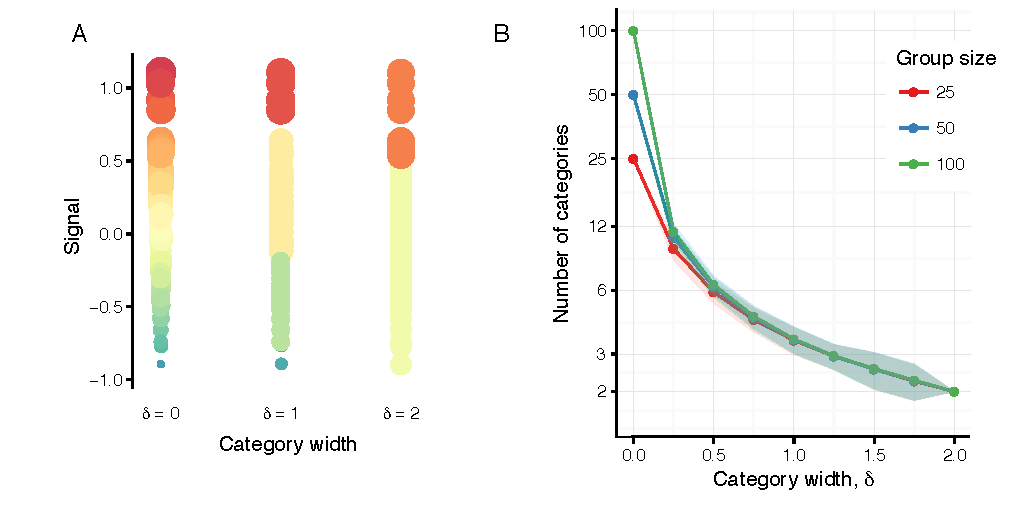
\includegraphics[width=.8\textwidth]{figures/category_diagram.pdf}
\caption{\sffamily\small\textbf{As category width increases, the animals use fewer categories, each of which includes more animals.} 
In A we show how a given set of signals could be categorized using three different category widths ($\delta$). The three vertical lines of dots represent the same group, with the same set of signals $\{s_i\}$. Each dot represents an animal in the group and the vertical position of a dot represents the animal's signal. In each column, animals in the same category are represented by circles of the same size and color, indicated the average signal for animals in that category. The range of signals in a given category can be no more than $\delta$. In the left column, $\delta=0$ and there are $N=100$ categories. In the middle column, $\delta=1$ and there are four categories. In the right column, $\delta=2$ and there are two categories.  In B, we show how the number of categories an animal uses depends on the category width. For a given group size ($N$) and category width, we generated $5,000$ groups with signal values $\{s_i\}$ and categorized the group according to the procedure shown in A.  Category width is on the x-axis. The average number of categories across the $5,000$ groups is on the y-axis, which is on a logarithmic scale, with the color indicating group size. The shaded areas show this average plus or minus the standard deviation across the $5,000$ groups. When $\delta=0$ there are as many categories as there are animals in the group. When $\delta=2$, it is theoretically possible for all animals to be put into the same category, but this was never observed, and instead the animals were always put into $2$ categories. }
 \label{category_diagram}
\end{figure}

\begin{figure}
%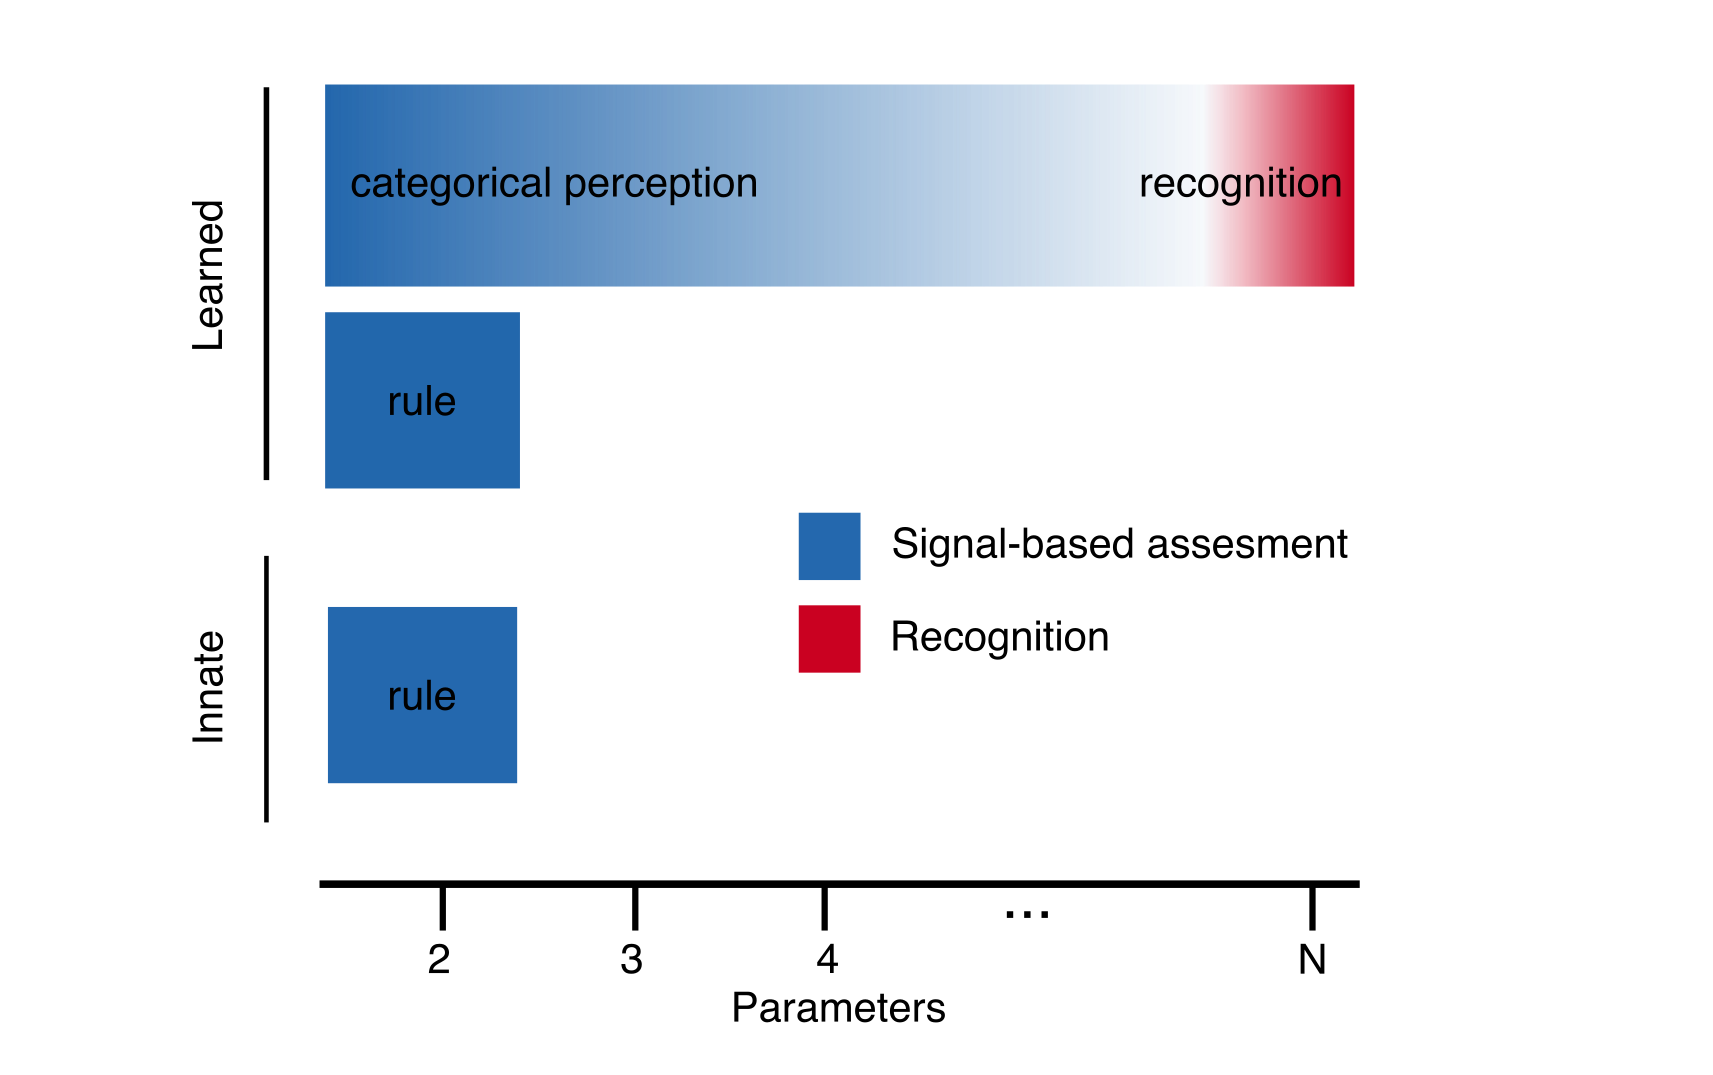
\includegraphics[width=6.85in]{figures/schematic_cropped.png}
\caption{\label{schematic}\sffamily\small\textbf{Animals can use signals to infer the quality values of conspecifics.} They can do so using either a linear rule, which can be either learned or innate and which is determined by a slope and intercept, or categories, which can be coarse or fine. When there are as many categories as there are individuals in the group, categorical perception becomes individual recognition.}
\end{figure}

\begin{figure}
%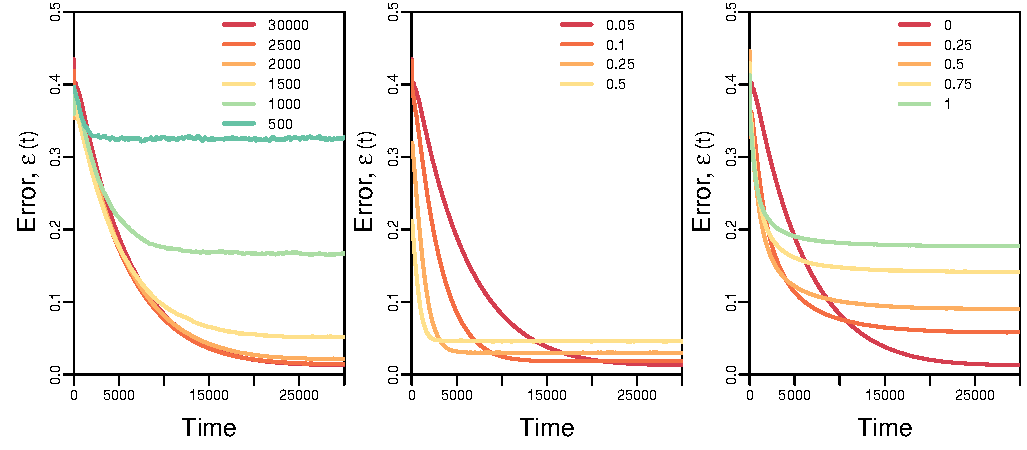
\includegraphics[width=6.85in]{figures/speed_accuracy_tradeoff.pdf}
\caption{\sffamily\small\textbf{As the animals learn, their errors decrease and eventually reach an equilibrium value.} Increasing the updating rate ($r$) or category width ($\delta$) helps the animals learn more quickly. When they have a long memory, this increases the equilibrium level of error, but when they have a short memory, it decreases the equilibrium level of error. In each panel, we show time ($t$, in number of interactions) on the x-axis and the average error in an animal's assessment of its peers ($\epsilon(t)$) on the y-axis. In each panel, light blue indicates animals using a learned rule, dark blue indicates animals using an innate rule, reddish colors indicates animals using recognition, and purple indicates animals using categorization. The points show the stopping time ($\tau$) at which error stops decreasing (not shown for the innate rule because there is no learning). In A and B, the different reddish curves represent different updating rates ($r$). In C and D, the red and purple curves represent different category widths ($\delta$). In the left column, memory window $w=2500$ and in the right column, memory window $w=500$. Parameters: unless the parameter is being varied $\delta=0$, $N=25$, $\rho=0.99$, $r=0.05$.}
\label{tradeoff}
\end{figure}

\begin{figure}
%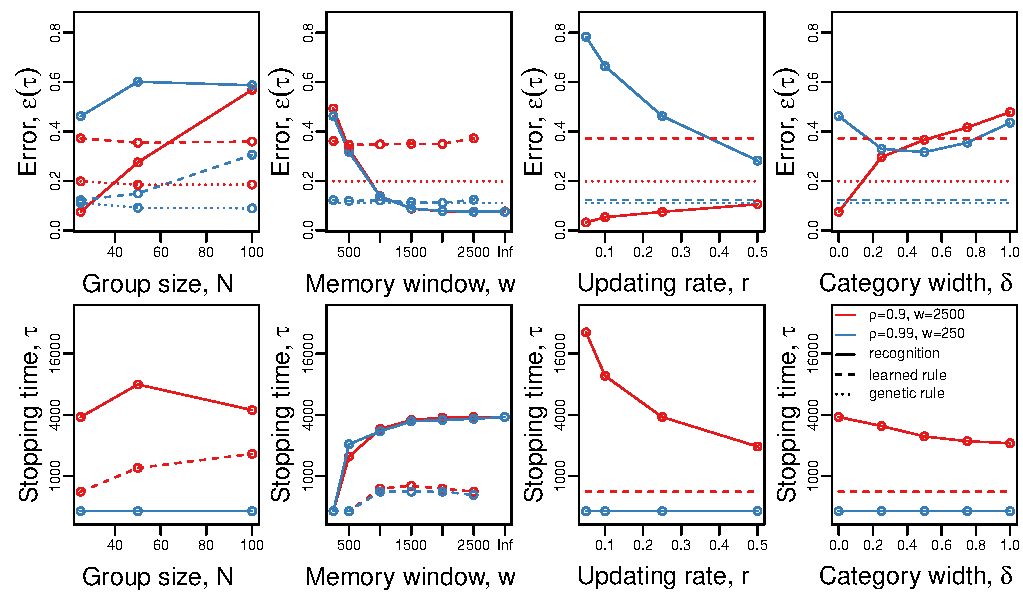
\includegraphics[width=6.85in]{figures/parameters_exploration.pdf}
\caption{\sffamily\small\textbf{Animals can learn about their peers with smaller errors when they have signals that are highly correlated with quality, live in small groups, and have long memory windows, and when errors are costly.} Here we show (A-D) average error ($\epsilon(\tau)$) and (E-H) stopping time ($\tau$) as a function of signal-quality correlation ($\rho$), group size ($N$), memory window ($w$), and cost of errors ($c$). Stopping time is on a logarithmic scale. In each panel, light blue curves show animals using a learned rule, dark blue curves show animals using a innate rule, red curves show animals using recognition ($\delta=0$), and purple curves show animals using categorization (with $\delta=0.25$). We do not show stopping time for animals using the innate rule because there is no learning involved.  The solid curves correspond to groups in which the signal-quality correlation $\rho=0.99$ and the dashed curves correspond to groups in which the signal-quality correlation $\rho=0.9$ (except in A and E, where we explicitly vary $\rho$). There are no dashed red curves because $\rho$ does not affect animals using recognition. Parameters: unless the parameter is being varied $c=1$, $N=25$, $r=0.5$, $w=2500$.}
\label{parameters}
\end{figure}

\begin{figure}
%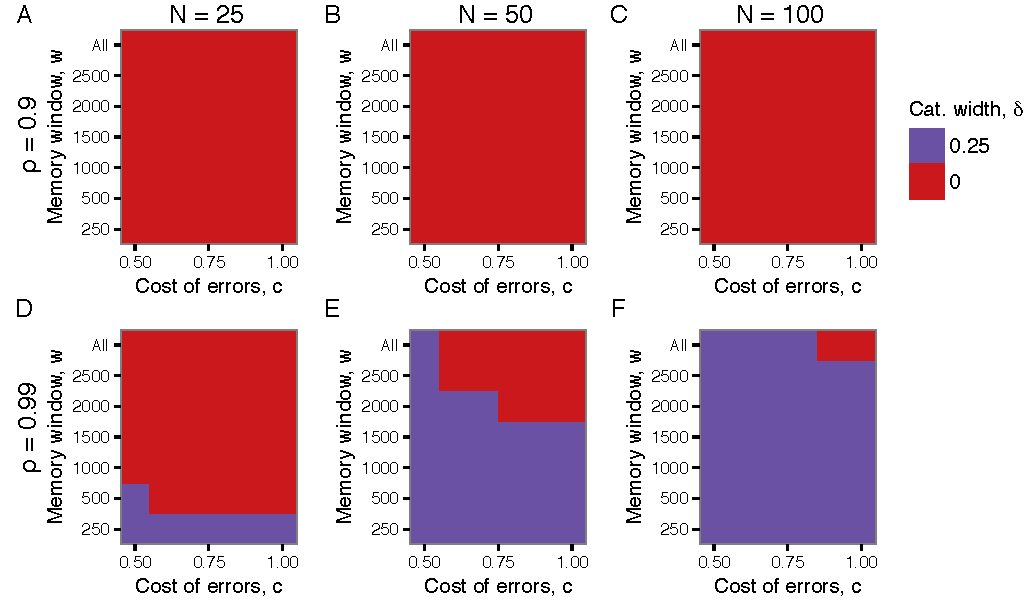
\includegraphics[width=6.85in]{figures/strategies_heat_maps.pdf}
\caption{\sffamily\small\textbf{Categorization is the better than recognition when animals live in large groups, have short memories, when the signal-quality correlation is high, and when errors are not very costly.} Here we show how the optimal category width ($\delta$), as a function of the cost of errors ($c$) and memory window ($w$). The optimal category width is the value of $\delta$ that minimizes the costs incurred from the combination of error and learning time. We concurrently find the value of $r$ that minimizes costs, as shown in Figure \ref{l}. In the first column, group size $N=25$, in the second column $N=50$, and in the third column $N=100$. Parameters: $\rho=0.99$. }
\label{optimization}
\end{figure}


\begin{figure}
%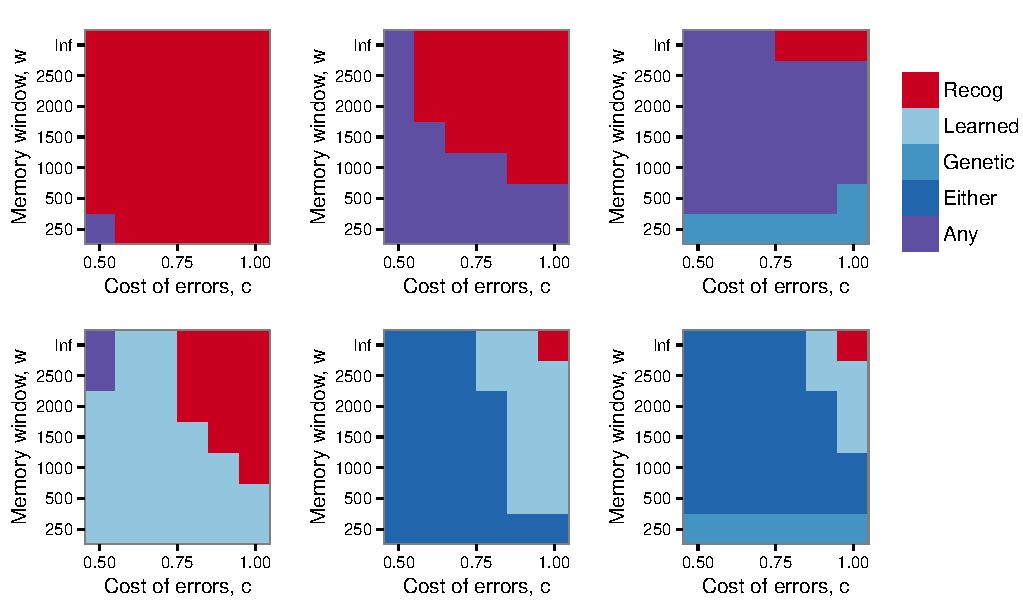
\includegraphics[width=6.85in]{figures/best_type_of_learning.pdf}
\caption{\sffamily\small\textbf{A rule is the best assessment strategy when animals live in large groups and have short memories, when the signal-quality correlation is high, and when errors are not very costly.} Here we show which of the three assessment strategies---recognition, a learned rule, or a innate rule---is the least costly, as a function of the cost of errors ($c$) and memory window ($w$). Red indicates recognition is the least costly. Light blue indicates a learned rule is the best strategy. Intermediate blue indicates a innate rule is the best strategy. Dark blue indicates the two rules are essentially equally costly and less costly than recognition. Grey indicates the three strategies are all essentially equally costly. (Strategies are classified as equivalent if their costs are within $0.05$ of each other.) Using categorization is never the least costly strategy. Animals using recognition are using the optimal stopping time ($\tau$), updating rate ($r$), and category width ($\delta=0$), as shown in Figures \ref{tau}-\ref{delta}, and animals using a learned rule are using the optimal stopping time. In the first column $N=25$, in the middle column, $N=50$, and in the right column $N=100$. In the first row $\rho=0.9$ and in the second row $\rho=0.99$.}
\label{best}
\end{figure}

%
\begin {table}[ht]
\caption {Description of variables} \label{tab:vars} 
\begin{tabular}{cl}

 Variables & Description of variables \\
\midrule 
$a_{ij}(t)$ & animal $i$'s assessment of animal $j$ at time $t$ \\
$C(t)$ & total cost of learning \\ 
$c$ & cost of errors, whereas $1-c$ is the cost of spending time learning \\ 
$\delta$ & category width (values near 0 = higher discriminatory ability, $\delta=0 \approx$ individual recognition)\\
$e_{ij}(t)$ & error of animal $i$ about animal $j$ at time $t$\\
$\epsilon(t)$ & average error of all animals in all groups at time $t$ \\
$N$ & number of animals in group (small=25, medium=50, large=100)\\ 
$\mathscr{O}_i(t)$ & set of animals about whom $i$ has an opinion at time $t$\\
$q_j$ & quality of animal $j$ \\ 
$\hat{q}_j$ & noisy information about the quality of animal $j$, $\hat{q}_j=q_j+\xi$ \\
$r$ & updating rate (values near 0 = very fast updating rates)\\
$\rho$ & sample correlation between quality and signal (high=0.9, almost perfect=0.99)\\
$s_j$ & quality signal of animal $j$ \\ 
$\sigma_\xi$ & standard deviation of noise in opinion updating during interaction, set to $0.1$ \\
$\sigma_\text{q}$ & standard deviation of quality values, set to $0.5$ \\
$T$ & total number of interactions, set to $30,000$ \\
$\tau$ & stopping time \\
$w$ & memory window (values near 0 = very short-term memory)\\
$\xi$ & noise in the information animals get about each other's quality through interacting
\end{tabular}
\end {table}



\newpage
\begin {table}[ht]
\renewcommand*{\arraystretch}{1.4}
\caption {Description of variables} \label{tab:vars2} 
\begin{tabular}[t]{ |c|c|l| }
  \hline
  \multirow{6}{*}{\rotatebox[origin=c]{90}{\parbox{2cm}{\centering Input \\ variables}}} 
  & $q_j$ 			& Quality of animal $j$ \\   
  & $\hat{q}_j$ 		& noisy information about the quality of animal $j$, $\hat{q}_j=q_j+\xi$ \\ 
  & $s_j$ 			& quality signal of animal $j$ \\ 
  & $\sigma_\xi$ 	& Standard deviation of noise in opinion updating during interaction, set to $0.1$ \\
  & $\sigma_\text{q}$ & Standard deviation of quality values, set to $0.5$ \\
  & $T$ 			& Total number of interactions, set to $30,000$ \\
  & $\xi$ 			& Noise in the information animals get about each other's quality through interacting \\
  \hline
  \multirow{5}{*}{\rotatebox[origin=c]{90}{\parbox{2cm}{\centering Parameters \\ manipulated}}} 
 	& $N$ & Number of animals in group (small=25, medium=50, large=100) \\
  & $\rho$ 		& Sample correlation between quality and signal (high=0.9, almost perfect=0.99)\\
  & $w$ 		& Memory window (values near 0 = very short-term memory, perfect memory $w=T$)\\
  & $\delta$ 	& Category width (values near 0 = higher discriminatory ability, $\delta=0 \approx$ individual recognition)\\
  & $r$ 		& Updating rate (values near 0 = very fast updating rates)\\
  \hline
  \multirow{7}{*}{\rotatebox[origin=c]{90}{\parbox{2cm}{\centering Output \\ variables}}} 
  & $a_{ij}(t)$ 		& Animal $i$'s assessment of animal $j$ at time $t$ \\
  & $\mathscr{O}_i(t)$ 	& Set of animals about whom $i$ has an opinion at time $t$\\
    & $e_{ij}(t)$ 		& Error of animal $i$ about animal $j$ at time $t$\\
  & $\epsilon(t)$ 		& Average error of all animals in all groups at time $t$ \\
  & $c$ 				& Cost of errors, whereas $1-c$ is the cost of spending time learning \\
  & $\tau$ 				& Stopping time \\
  & $C(t)$ 				& Total cost of learning \\ 

  \hline
\end{tabular}
\end {table}





%%%%%%%%%%%%%%%%%%%%%% FIGURES
\clearpage
\setcounter{figure}{0}

\begin{figure}
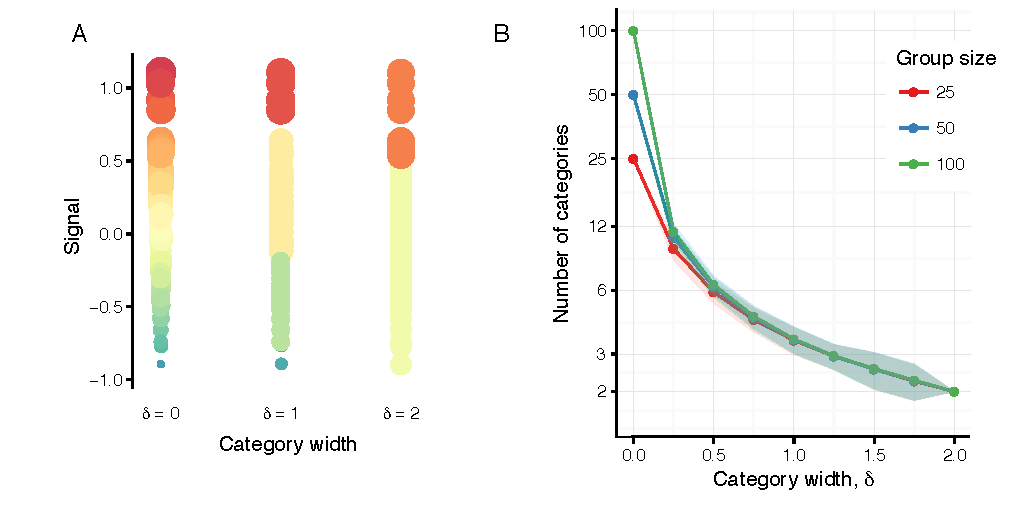
\includegraphics[width=6.85in]{figures/category_diagram.pdf}
\caption{}
\end{figure}

\begin{figure}
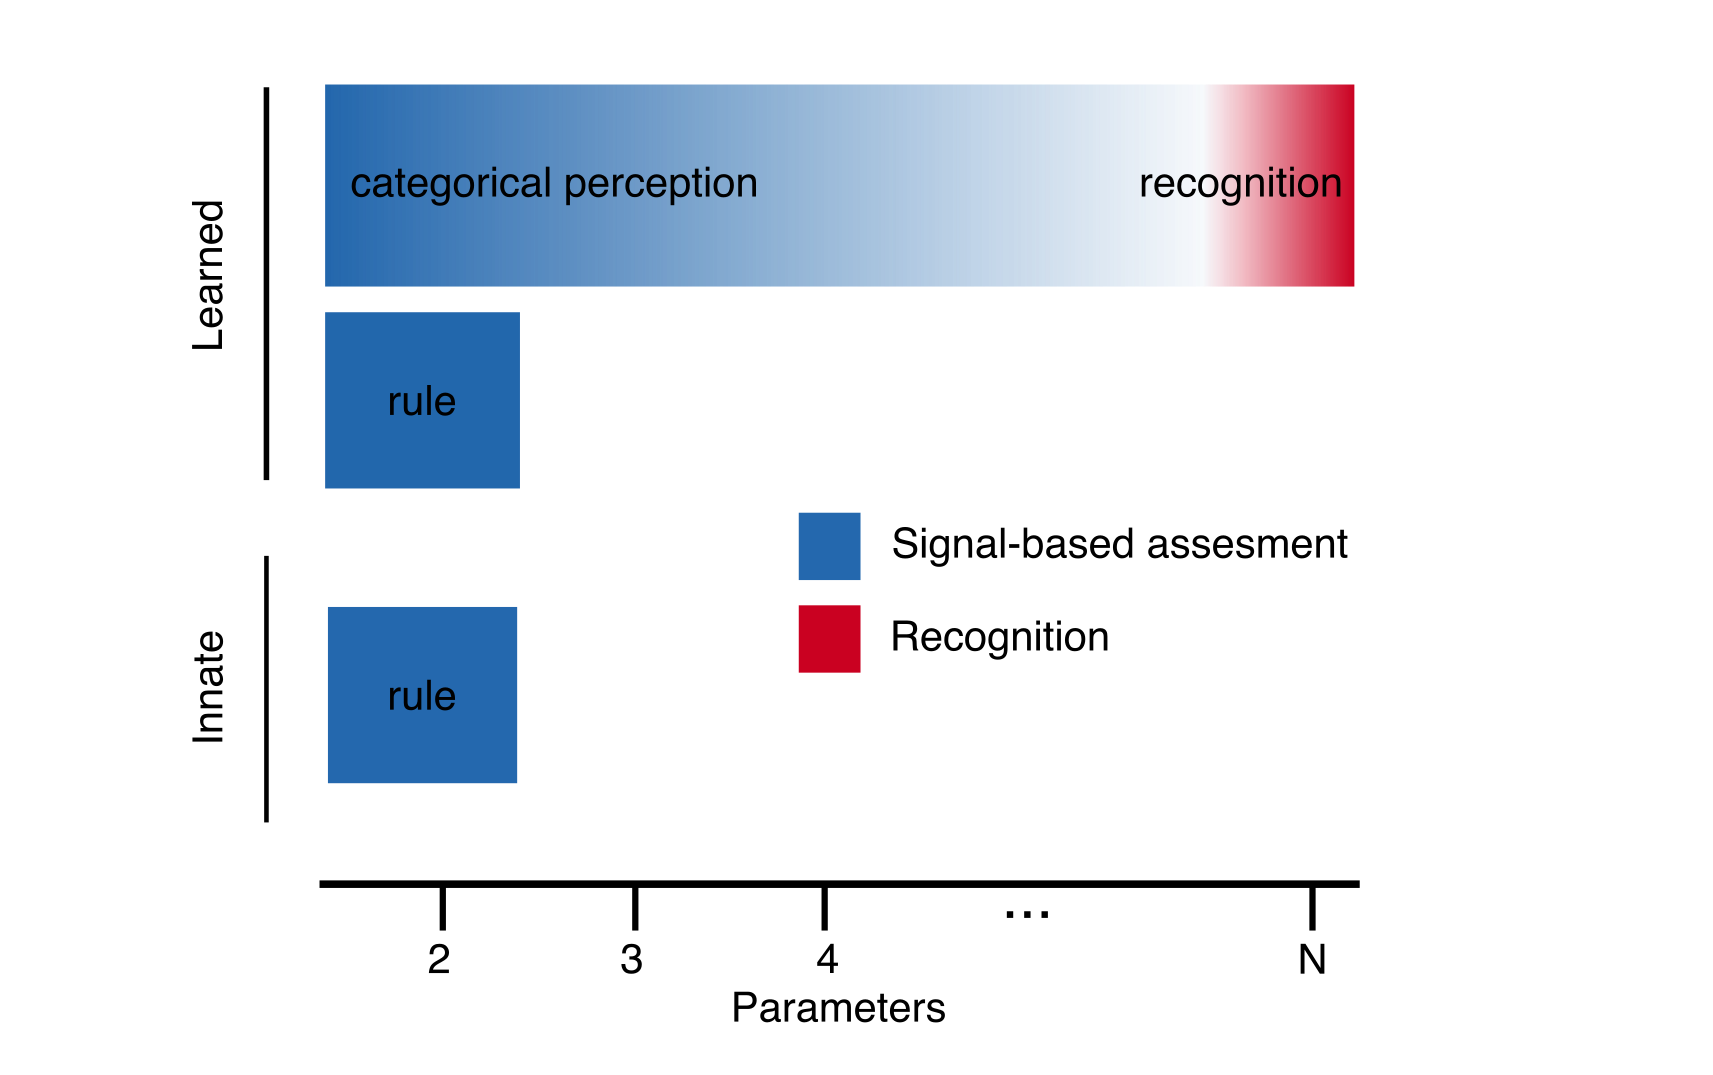
\includegraphics[width=6.85in]{figures/schematic_cropped.png}
\caption{}
\end{figure}

\begin{figure}
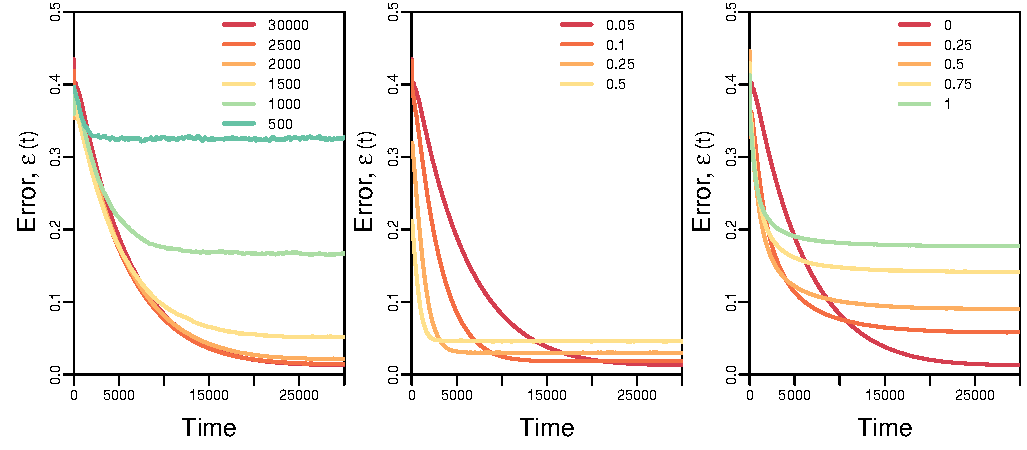
\includegraphics[width=6.85in]{figures/speed_accuracy_tradeoff.pdf}
\caption{}
\end{figure}

\begin{figure}
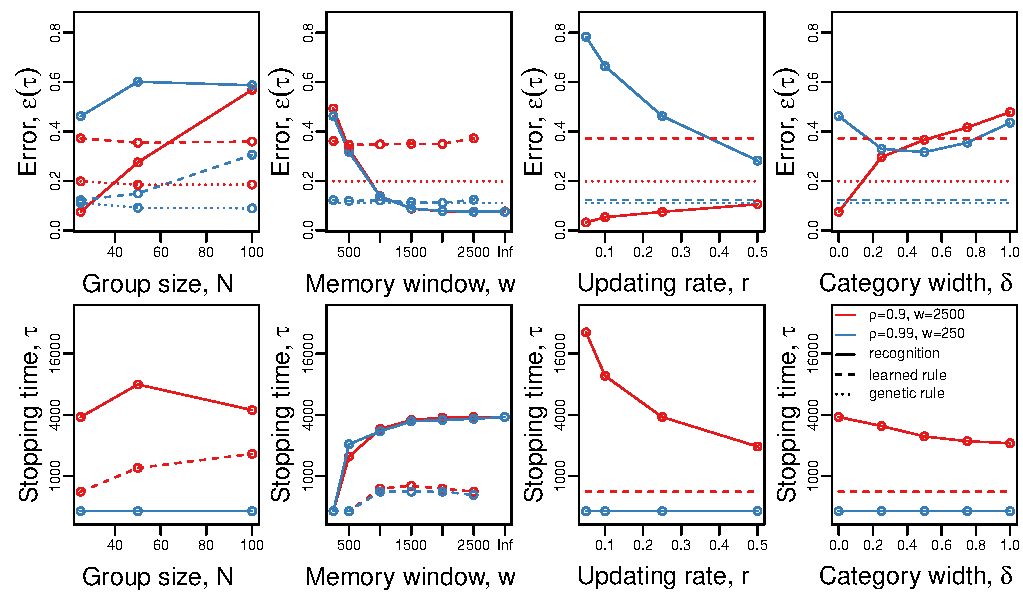
\includegraphics[width=6.85in]{figures/parameters_exploration.pdf}
\caption{}
\end{figure}


\begin{figure}
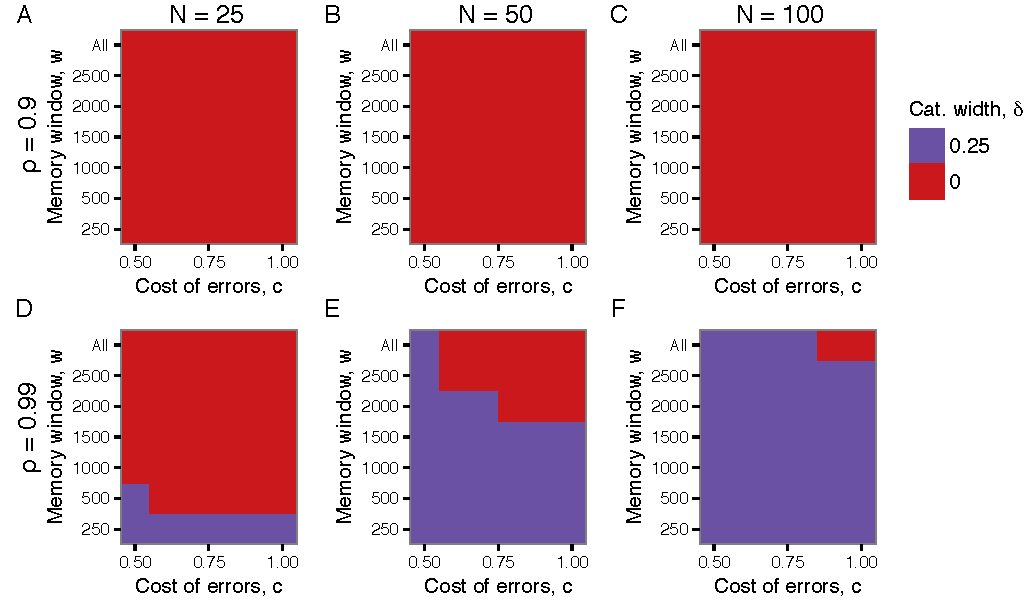
\includegraphics[width=6.85in]{figures/strategies_heat_maps.pdf}
\caption{}
\end{figure}


\begin{figure}
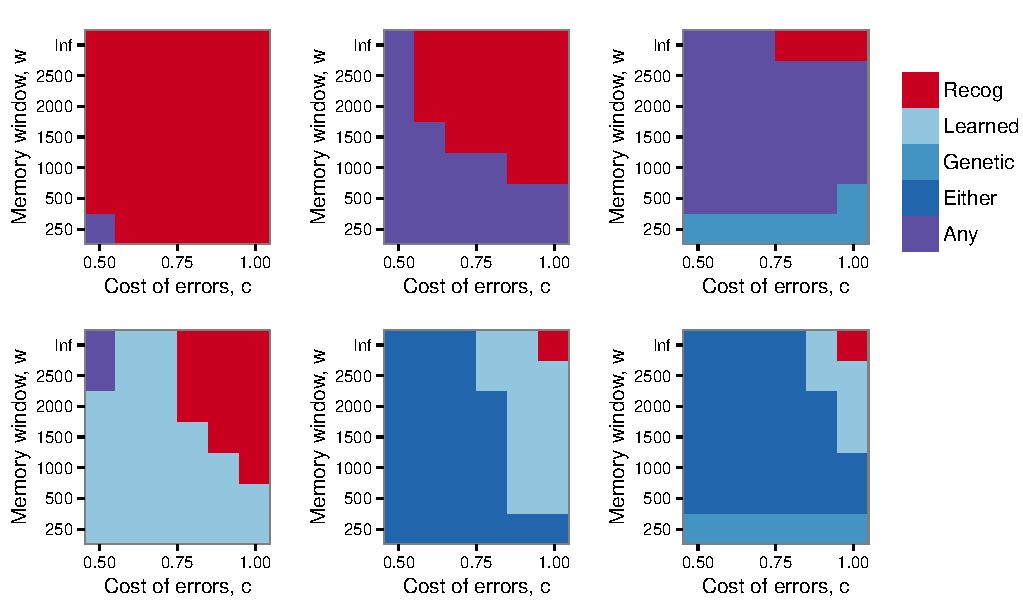
\includegraphics[width=6.85in]{figures/best_type_of_learning.pdf}
\caption{}
\end{figure}

\clearpage{}
%\newpage{}
\renewcommand{\thesection}{}
\section{Supporting information}
\renewcommand{\thesection}{S}
\renewcommand{\thesubsection}{S\arabic{subsection}}
\renewcommand{\theequation}{S\arabic{equation}}
\renewcommand{\thetable}{S\arabic{table}}
\renewcommand{\thefigure}{S\arabic{figure}}
\setcounter{equation}{0}  
\setcounter{figure}{0}
\setcounter{table}{0}

\begin{figure}[ht]
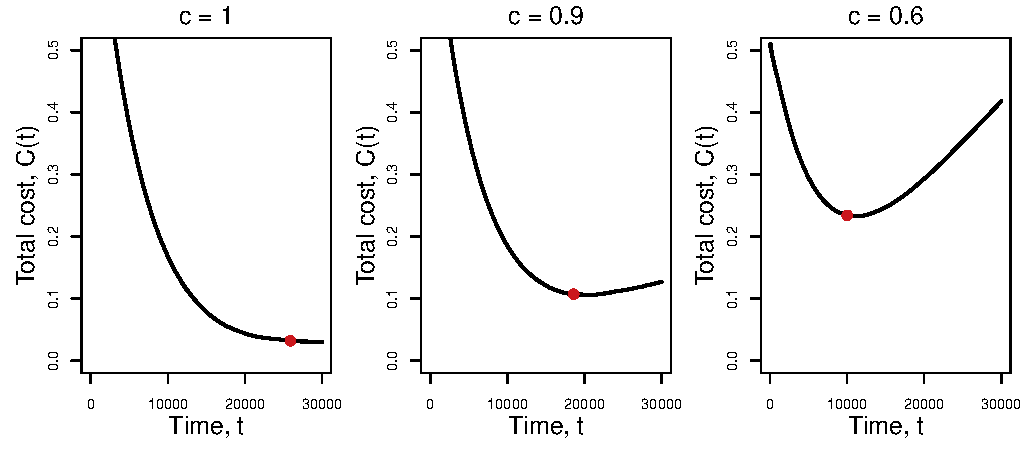
\includegraphics[width=6.85in]{figures/stopping_time.pdf}
\caption{\sffamily\small\textbf{As the cost of errors decreases and the cost of learning time increases, animals should stop learning earlier.} Here we show how we calculate stopping time ($\tau$). In each panel, time in number of interactions ($t$) is on the x-axis and the total cost $C(t)$ is on the y-axis. In A, the cost of errors $c=1$: all that matters is error and the total cost $C(t)$ is equal to $2$ times the average error $\epsilon(t)$. In B, the cost of errors $c=0.9$ and in C, the cost of errors $c=0.6$: in each case, as time goes on, the animals incur costs from their interactions. In each panel, the stopping time $\tau$ is shown with the red point: this is the number of interactions at which the cost $C$ stops decreasing and either plateaus or starts to increase. Parameters: $\delta=0$, $N=25$, $\rho=0.9$, $r=0.05$, $w=2500$.)
}
\label{tau}
\end{figure}


\begin{figure}[ht]
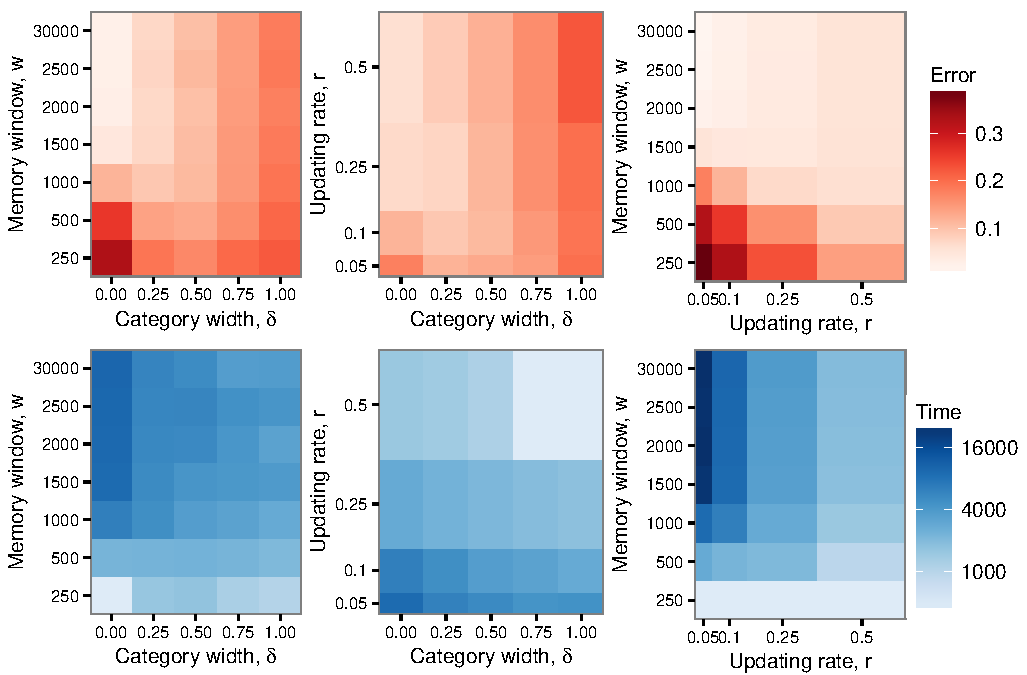
\includegraphics[width=6.85in]{figures/parameters_interactions_full.pdf}
\caption{\sffamily\small\textbf{Memory window, updating rate, and category width interact in their effects on how quickly and accurately animals using categorization can learn.}
Here we show stopping time ($\tau$) (A-C) and average error ($\epsilon(\tau)$) (D-F) for animals using categorization as a function of two parameters. Stopping time is on a logarithmic scale. Increasing memory window increases stopping time (A and C) and decreases error (D and F). Increasing category width decreases stopping time (A and B). Intermediate category widths minimize error when memory and updating rate are low, but otherwise category width $\delta=0$ minimizes error (D and E). Increasing updating rate decreases stopping time (B and C). When memory window is low, increasing updating rate decreases error, but when memory window is high, increasing updating rate \emph{increases} error (F). Parameters: unless the parameter is being varied $\delta = 0$, $N=25$, $\rho=0.99$, $w=1000$, $r=0.1$. 
}
\label{interactions}
\end{figure}

\begin{figure}
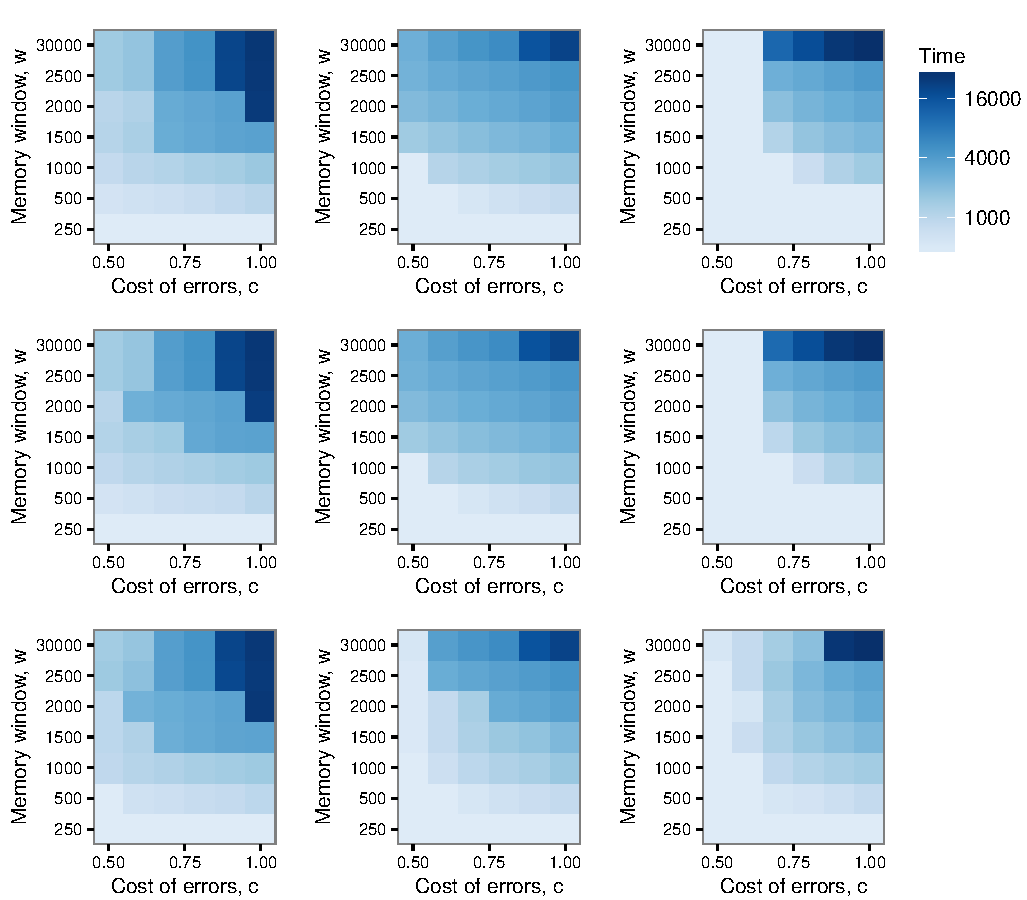
\includegraphics[width=6.85in]{figures/time_heat_maps.pdf}
\caption{\sffamily\small\textbf{} Here we show how the optimal stopping time ($\tau$) depends on the cost of errors ($c$) and memory window ($w$). Stopping time is on a logarithmic scale. In the first column $N=25$, in the middle column $N=50$, and in the right column $N=100$. In the first row $\rho=0.5$, in the second row $\rho=0.9$ and in the third row $\rho=0.99$. The animals are also using the optimal updating rate ($r$) and category width ($\delta$), which are shown in Figures \ref{delta} and \ref{l}.}
\label{time}
\end{figure}

\begin{figure}
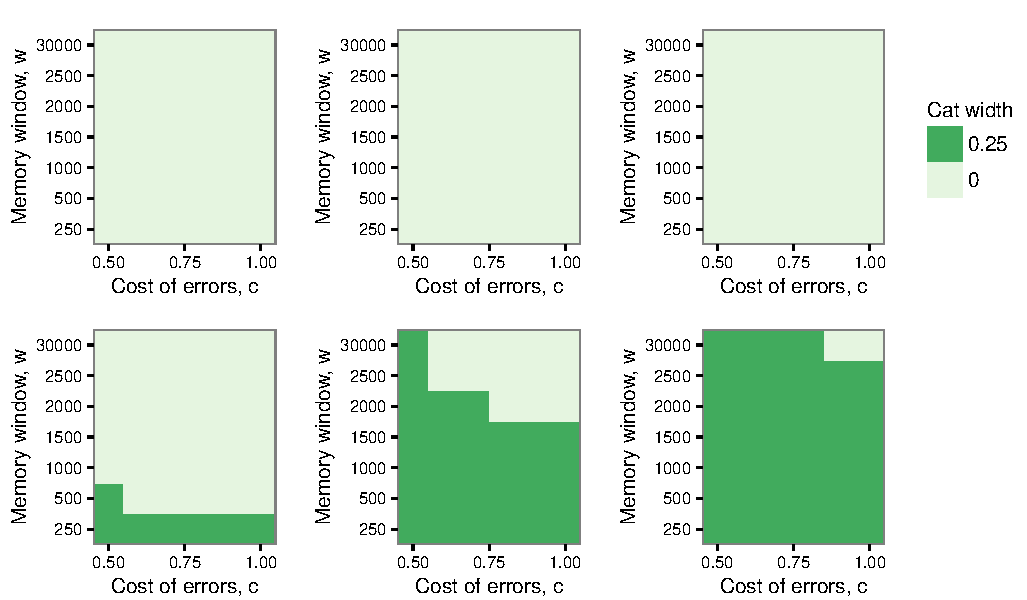
\includegraphics[width=6.85in]{figures/delta_heat_maps.pdf}
\caption{\sffamily\small\textbf{Categorical recognition is better than individual recognition when animals live in large groups and have short memory windows and when the signal-quality correlation is very high.} Here we show how the optimal category width ($\delta$) depends on the cost of errors ($c$) and memory window ($w$). In the first column $N=25$, in the middle column $N=50$, and in the right column $N=100$. In the first row $\rho=0.5$, in the second row $\rho=0.9$, and in the third row $\rho=0.99$. The animals are also using the optimal stopping time ($\tau$) and updating rate ($r$), which are shown in Figures \ref{time} and \ref{l}.}
\label{delta}
\end{figure}

\begin{figure}
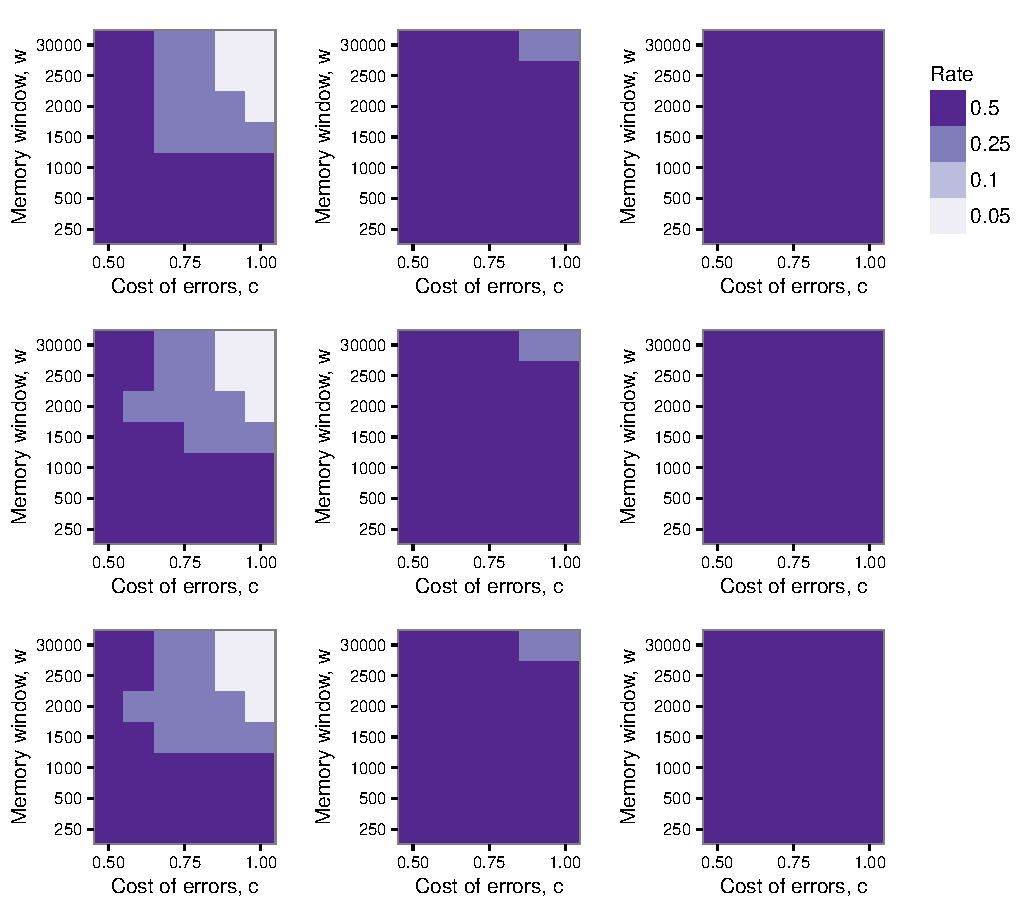
\includegraphics[width=6.85in]{figures/l_heat_maps.pdf}
\caption{\sffamily\small\textbf{A high updating rate is better than a low updating rate when animals live in large groups and have short memory windows.} Here we show how the optimal updating rate ($r$) depends on the cost of errors ($c$) and memory window ($w$). In the first column $N=25$, in the middle column $N=50$, and in the right column $N=100$. In the first row $\rho=0.5$, in the second row $\rho=0.9$, and in the third row $\rho=0.99$. The animals are also using the optimal stopping time ($\tau$) and category width ($\delta$), which are shown in Figures \ref{time} and \ref{l}.}
\label{l}
\end{figure} 

\begin{figure}
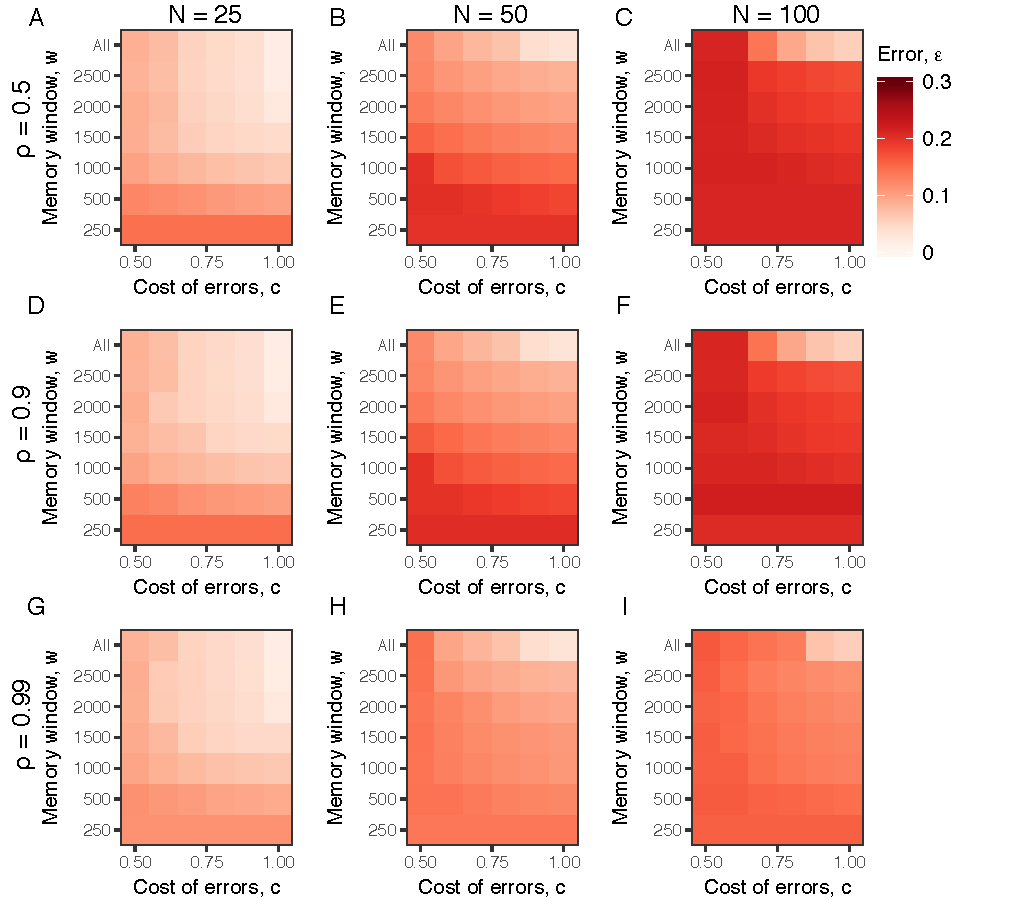
\includegraphics[width=6.85in]{figures/error_heat_maps.pdf}
\caption{\sffamily\small\textbf{} Here we show how the average error ($\epsilon(\tau)$) of animals using optimal stopping time ($\tau$), updating rate ($r$), and category width ($\delta$), depends on the cost of errors ($c$) and memory window ($w$). In the first column $N=25$, in the middle column $N=50$, and in the right column $N=100$. In the first  row $\rho=0.5$, in the second row $\rho=0.9$ and in the third row $\rho=0.99$.}
\label{error}
\end{figure}

\begin{figure}
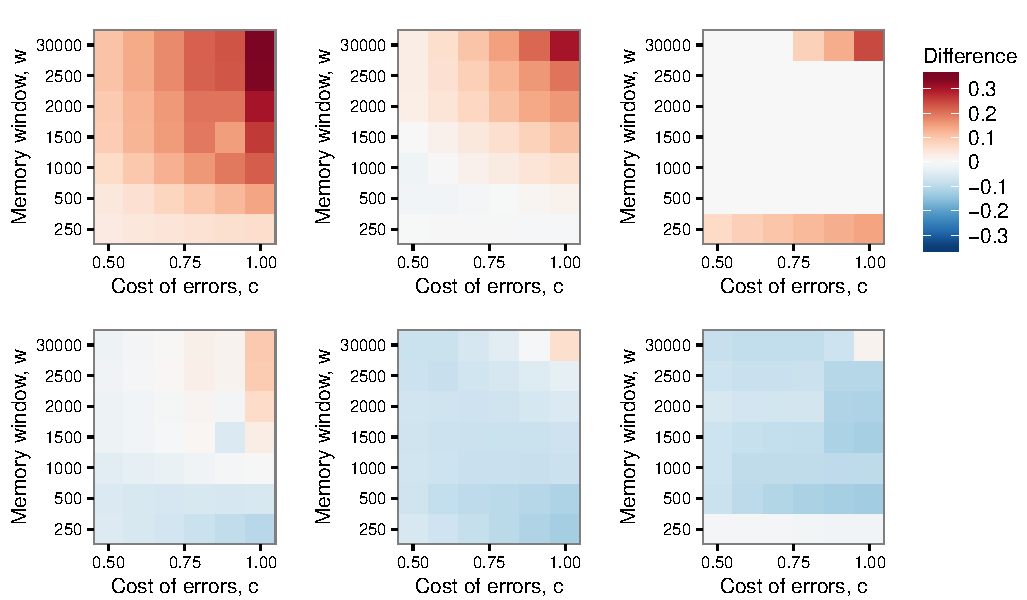
\includegraphics[width=6.85in]{figures/recog_vs_learned_rule.pdf}
\caption{\sffamily\small\textbf{A learned rule is less costly than recognition (with optimized learning strategies) when animals live in large groups and have short memories and when the signal-quality correlation is high.} In each panel, we show the difference in overall costs between recognition and a learned rule as a function of the cost of errors ($c$) and memory window ($w$). Blue indicates a learned rule is less costly and red indicates recognition is less costly. The animals using recognition are using the optimal stopping time ($\tau$), updating rate ($r$), and category width ($\delta$). In the first column $N=25$, in the middle column, $N=50$, and in the right column $N=100$. In the first row $\rho=0.9$ and in the second row $\rho=0.99$.}
\label{comparison}
\end{figure}

\begin{table}
\caption{\label{corr_examples} Examples of the correlation between a badge and a measure of fitness.}
\begin{tabular}{lllll}
Species & Badge & Measure of fitness & Correlation & Reference
\\\hline paper wasp & percent black on face & head width & $r^2=0.36$, for wasps  & Tibbetts \& Dale 2004
\\ & & & with $\geq 2$ black spots
\\ & ``badge brokenness" & dominance & $r^2=.105$ & Tibbetts \& Dale 2004
\\ \hline house sparrow & size of black bib & physical condition & $r=0.379$ & Veiga 1993
\\ \hline swamp sparrow & size of rusty cap & parental investment & $r^2=0.33$ & Olsen et al. 2010
\\ & size of black forehead & aggression & $r^2=0.41$ & Olsen et al. 2010
\end{tabular}
\end{table}

\end{document}
